\documentclass[12pt, a4paper]{article}
\usepackage{graphicx}
\usepackage{multicol}
\usepackage{blindtext}
\usepackage{float}
\usepackage{placeins}
\usepackage{url}
\title{PM2.5 Incidence and Access to Green Spaces in relation to Income Inequality in Eindhoven}
\author{Guilherme Oliveira}
\date{\today}
\begin{document}
\maketitle
\begin{abstract}
    While environmental concerns are often addressed on a global scale, their local and unequal impacts remain underexplored. Understanding how climate-related factors like PM2.5 exposure and access to green spaces vary across income levels can help inform equitable public health and urban planning policies. However, research on the intersection of air pollution, green space access, and income inequality at the municipal level is still limited. This study aims to examine whether income inequality correlates with levels of air pollution and access to green spaces across neighborhoods in Eindhoven, Netherlands. Data were collected from publicly available municipal datasets and processed using Python, geospatial tools, and machine learning models including Random Forest and Gradient Boosting Regressors. The findings reveal a strong correlation between income and access to green spaces, with lower-income neighborhoods having significantly reduced access. However, no consistent pattern was found linking income levels to PM2.5 exposure. The best-performing model achieved a low predictive accuracy (R² = 0.02), highlighting the need for more comprehensive data. These results suggest that while green space inequality is evident, the relationship between income and pollution is more complex. Urban policymakers should prioritize equitable green infrastructure in low-income areas and improve data transparency to better address environmental disparities.
\end{abstract}
\begin{multicols}{2}
    \section{Introduction}
    PM2.5 and other classifications of air pollution are a pressing issue often dismissed in the public discourse. However, the effects of air pollution need not just be further explored and researched but also reiterated and emphasised to the public, as PM2.5 pollution becomes more and more of a problem in public health.
    PM2.5 as air pollution has significant impact on asthma patients, in respiratory inflammation, lung function and is a known carcinogen. All of these effects have an impact on life expectancy; in the European Union, it decreased the average life span by 8.6 months \cite{xing2016impact}. Another source points to an estimated 5.8\% increase in deaths \cite{Schwartz01101996}. According to the World Health Organisation, PM2.5 is responsible for 4.2 million premature cardiovascular, respiratory and cancer deaths \cite{THURSTON2022107066}.
    Tangential to this issue are the significant inequalities in exposure to pollution and other factors, which access to green spaces will tackle and analyse in this report.  Because rooted in the choice of researching and writing about this topic is the acknowledgement that technical skills like Machine Learning and Data Science can be used to advise public policy and keep governments accountable for their inaction while also starting a conversation about topics which are on the public interest. Thusly, to research a topic such as the relation between income inequality, PM2.5 and access to green spaces in my local community of Eindhoven, becomes a way of activism and utilising skills which would be otherwise utilised for profit gains becomes a form of activism.
    As such, I justify this research as a way to highlight potential inequalities in Eindhoven and proactively advise the local government to conduct further investigation and action to minimise these inequalities.
    PM2.5 are particles smaller than 2.5~\(\mu\)m, although the chemical composition of the particles is not taken into account when categorising. W. Gene Tucker highlights that not every particle is the same when it comes to its effects on human exposure. Access to green spaces and especially their maintenance and proximity to residency is an important factor for public health. Yet, it is an unknown factor, despite how important it would be to highlight and solve it, if income inequality has any effect on PM2.5 exposure and access to green spaces. Understanding the relation between wealth inequality and factors related to public health is important because, if the hypothesis that lower income neighborhoods are more exposed to PM2.5 and have less access to green spaces could mean that communities which have less money to spend on health care could be more exposed to conditions which could warrant expensive treatment or debilitation in labour capacity, therefore making them even more vulnerable. Lower income communities often also suffer from more stress, and therefore would be the ones for which access to green spaces is most crucial for relaxation and community building. This research is necessary because these inequalities must be highlighted in order to build a more fair, equitable society.
    The main research question is: \textbf{Is there a correlation between air pollution exposure (PM2.5 and Nitrogen Dioxide), income inequality and access to green spaces in Eindhoven?}
    The research question will be asked using machine learning and data analysis techniques to analyse public datasets. Based on the results, this report will provide direct advice on what the local government of Eindhoven should do to mitigate the issue. With such efforts, this study aims to achieve change in attenuating social inequalities.
    \section{Methodology}
    In order to find if there is a correlation between PM2.5 and access to green spaces with income, the data must be collected, cleaned, preprocessed, analysed and then played with using different machine learning (ML) models. These methods will be described in length in this section of the report.
    \subsection{Data Collection}
    The data was collected from publicly available datasets accessible via the municipality's website, in the Open Data section. There are 4 datasets which were relevant enough to collect:
    \begin{itemize}
        \item Air Pollution data (PM2.5, along with PM10, PM1 and Nitrogen Dioxide), which also contain geographical data for each sensor and timestamp. This data was requested to the platform which consumes the API that the municipality uses. A script was created to request the data from 2021 to 2025 by using Selenium to navigate the website and change the timespan \cite{eindhoven_pm25_data}. For replication purposes, refer to the script-csvs.py script in the repository. Another script was composed to merge all of those tiny datasets in a larger dataset by separating the header rows and the value rows, getting the columns and, while iterating for each sensor, filling in the columns with the correct values. The merged dataset ends up containing all the data from those small datasets in one, with a frequency in records of 1 day per sensor.
        \item Income per neighborhood data, which contains the average income per capita per neighborhood in Eindhoven throughout the years. \cite{eindhoven_incijfers}
        \item Green spaces data, which contains geographical data for each green space, along with year of construction, size and neighborhood. \cite{eindhoven_groen_data}
        \item Neighborhood Geographical Location data, so it can be merged with the income per neighborhood data, which only contains the name of the neighborhood. \cite{eindhoven_buurten_data}
    \end{itemize}
    All of the datasets were downloaded in CSV format.
    All quality of data is the responsibility of the municipality.
    \subsection{Data Cleaning}
    All data was cleaned using Python and the Pandas library.
    No treatment was done to the income data, as it was already clean enough for the purposes of this analysis.
    \subsubsection{Air Pollution Data}
    Upon being loaded into a DataFrame, numerical columns like Latitude, Longitude, PM1, PM2.5 and PM10 shall be converted into a numerical value, and the original separation by comma is replaced by a dot, for easier processing. Local time is converted into a datetime type, and UTC time is dropped.
    From a list of essential columns, like SensorID, PM1, PM2.5 and PM10, all the null values should be dropped. The DataFrame is then grouped by Sensor and all values are resampled by year and aggregated with statistical summaries (mean, median, standard deviation (std), min and max).
    After saving the dataset manually, the neighbourhoods are added into the csv file based on their ID and the map available at the municipality's website \cite{eindhoven_realtime_pm_data}. Once that manual task is done, it's loaded back again into a DataFrame; all the rows without a neighbourhood should be dropped. The dataset with neighbourhood data is loaded into its own DataFrame, and based on the name of the neighbourhood, the latitude, longitude and coordinates are added to the air pollution DataFrame. This is done by mapping each Sensor ID to a Neighbourhood and getting their geographical data. Thusly, each record gets their added geographical data based on the SensorID.
    \subsubsection{Green Spaces Data}
    The csv file is loaded into a DataFrame. The geographical points are split into Latitude and Longitude columns, where they are then converted into numerical values. The geographical points and shape columns, along with street and technique columns, are dropped out of the DataFrame as they are deemed unnecessary for the analysis.
    \subsection{Data Preprocessing}
    The air pollution dataset unfortunately does not encompass all the neighbourhoods in Eindhoven. So, in order to make a more complete analysis of how income per neighbourhood relates to air pollution exposure, data enhancement is employed. Two techniques were used in combination: computing the missing values using Inverse Distance Weighting (IDW) and predicting the values using a Random Forest Regressor. The use of both techniques in tandem is to ensure better accuracy and that the values better reflect real life. It is important to note that the values are not exact but hopefully are approximate enough to be useful for comparison with other neighbourhoods and correlation analysis.
    At first, the air pollution dataset (after cleaning) and the neighborhoods dataset are loaded. Then the missing neighborhoods are identified by checking which neighborhoods are not present in the air pollution dataset. Then IDW is applied to estimate the air pollution values for the missing neighborhoods based on the values from neighbouring locations. Essentially, the missing values are computed according to the following formula: 
    \begin{equation}
        \hat{v}(x, y) = \frac{\sum_{i=1}^n \frac{v_i}{d_i^p}}{\sum_{i=1}^n \frac{1}{d_i^p}}  
    \end{equation}
    where $d_i^p$ is the Haversine Distance.

    The formula describes the Inverse Distance Weighting (IDW) method, where $\hat{v}(x, y)$ is the estimated value at the point $(x, y)$, $v_i$ are the known values at the points $i$, $d_i$ is the distance from the point $(x, y)$ to the point $i$, and $p$ is a power parameter that determines how much influence nearby points have on the estimated value. In this case, $p$ is set to 2, which means that closer points have a greater influence on the estimated value than farther points.

    Upon these computations, the same process is repeated, but instead of applying IDW, a Random Forest Regressor model is trained for every column in the original dataset and used to predict the missing neighbourhoods.
    After both of these processes, the mean of the two separate predictions is calculated and taken as the value for the previously unknown neighborhoods. Forethermore, the DataFrame with the real values is concatenated to the new DataFrame, so the real values stay intact.
    \subsection{Machine Learning Models}
    All models tested and trained used as target the income of a neighborhood in 2022, because that's when the dataset is most complete, and total green space, number of green areas, average size of green areas, distance to green spaces, Mean of PM2.5, Mean of PM10 and Mean of NO2 as features. The air pollution dataset is grouped by Neighborhood and aggregated by the mean for PM2.5, PM10, NO2 and coordinates.
    The green spaces dataset is grouped by neighborhood and aggregated by the sum, count and mean for surface area. The distance between each neighborhood and the nearest green space is also calculated.
    All datasets are then merged into one.

    All features are scaled using a Standard Scaler and the dataset is split using an 80/20 split, with 80\% of the data being used for training and 20\% for testing. The models are trained using the training set and evaluated using the test set.
    The following models were tested:
    \begin{itemize}
        \item Linear Regression
        \item Ridge Regression (alpha = 1.0)
        \item Lasso Regression (alpha = 0.1)
        \item Random Forest Regressor (100 estimators)
        \item Gradient Boosting Regressor (100 estimators)
        \item Support Vector Regressor (SVR) \\ (kernel = "rbf", C = 100)
        \item K-Nearest Neighbors Regressor (5 neighbors)
        \item K Means Clustering (4 clusters)
    \end{itemize}
    Models were evaluated using $R^2$, which describes the influence that features have on the target, and Root Mean Squared Error (RMSE).
    \section{Results}
    The following table lays out the results by model, with respective evaluation metrics:
    \begin{table}[H]
    \caption{Evaluation metrics by model}
    \setlength{\tabcolsep}{4pt} 
    \begin{tabular}{|l|r|r|}
        \hline
        Model & $R^2$ & RMSE \\
        \hline
        Linear Regression & -0.21 & 18.41 \\
        Ridge & -0.21 & 18.38 \\
        Lasso & -0.22 & 18.49 \\
        Random Forest & 0.02 & 16.57 \\
        Gradient Boosting & -0.09 & 17.49 \\
        SVR & 0.03 & 16.46 \\
        KNN & -0.23 & 18.55 \\
        \hline
    \end{tabular}
    \end{table}
    \FloatBarrier
    
    When looking at the best performing model that can provide us with a feature importance score, which is the Random Forest Regressor, the results are as plotted on this graph:
    \begin{figure}[H]
        \centering
        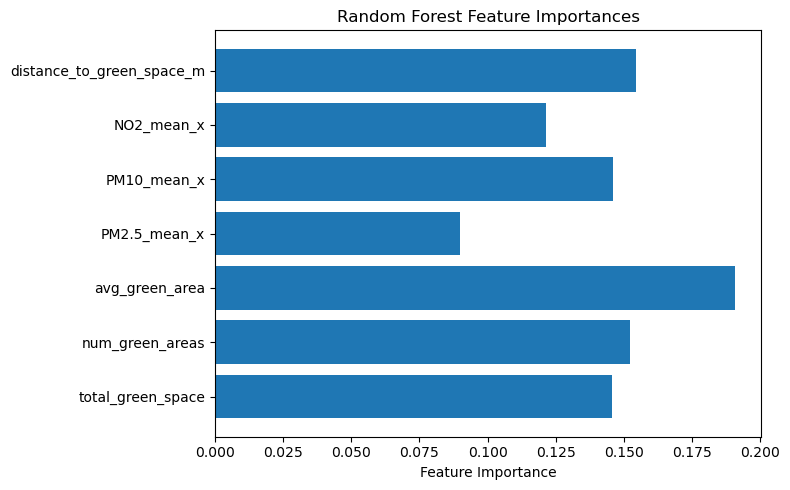
\includegraphics[width=0.45\textwidth]{../Images/feature_importance.png}
        \caption{Feature importance by Random Forest Regressor}
        \label{fig:feature_importance}
    \end{figure}

    Figure 1 quantifies how important a feature is for the model to predict the output, in this case, the income of a neighborhood in 2022. The plot shows that the most important features are the average size of a green area, the number of green areas and the distance to a green space.
    Upon KMeans clustering (on 4 clusters), the following clusters were found:
    \begin{figure}[H]
        \centering
        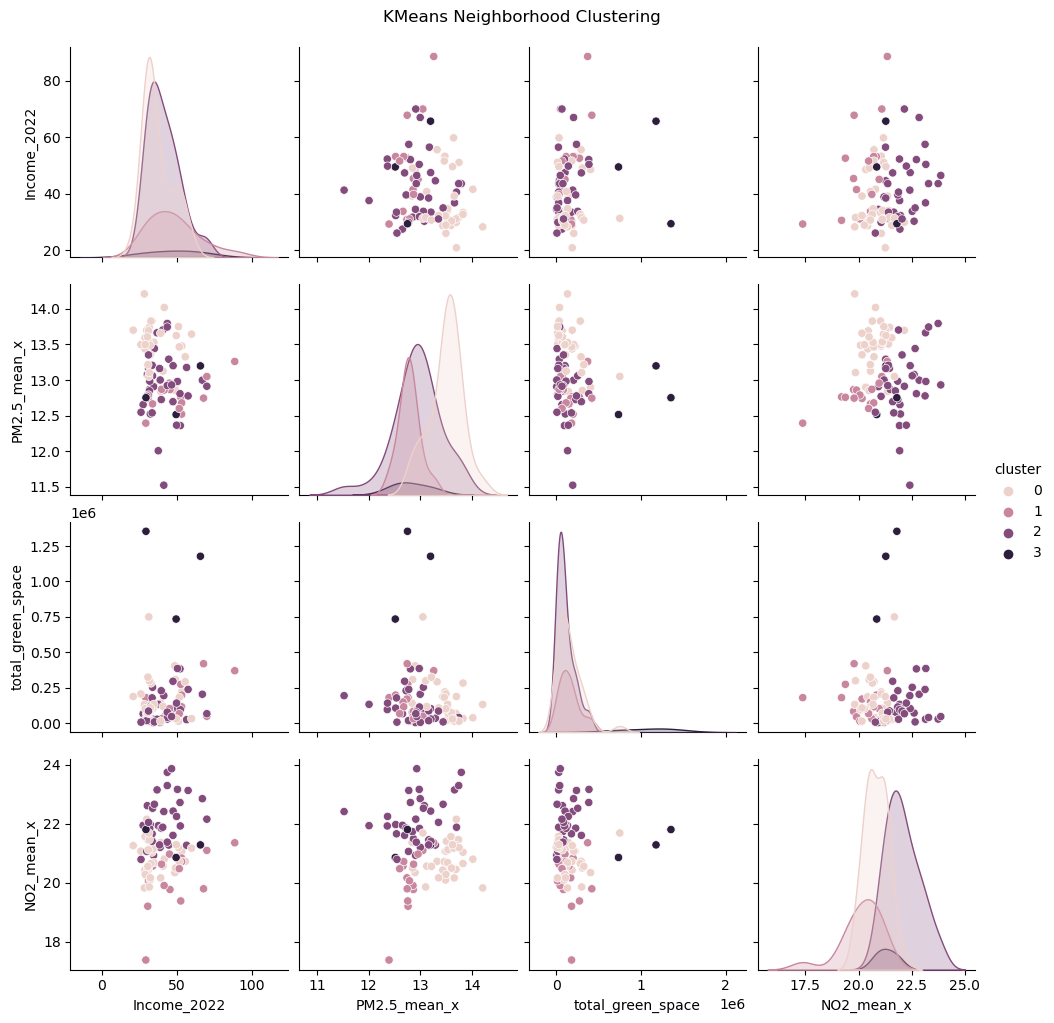
\includegraphics[width=0.45\textwidth]{../Images/kmeans_clusters.png}
        \caption{KMeans Clusters}
        \label{fig:kmeans_clusters}
    \end{figure}

    Figure 2 tells us about 4 distinct clusters which represent different neighbourhoods according to their relation with income, air pollution and access to green spaces.
    Cluster 0 has lower air pollution and moderate to low income. However, it has low access to green spaces.
    Cluster 1 is a low income neighborhood with poor access to green spaces and elevated levels of air pollution.
    Cluster 2 has moderate income with high air pollution and some of the lowest green space access.
    Cluster 3 has the highest income, also high levels of air pollution and high access to green spaces.

    The map below represents each neighbourhood in Eindhoven, with the clusters represented by different colours:
    \begin{figure}[H]
        \centering
        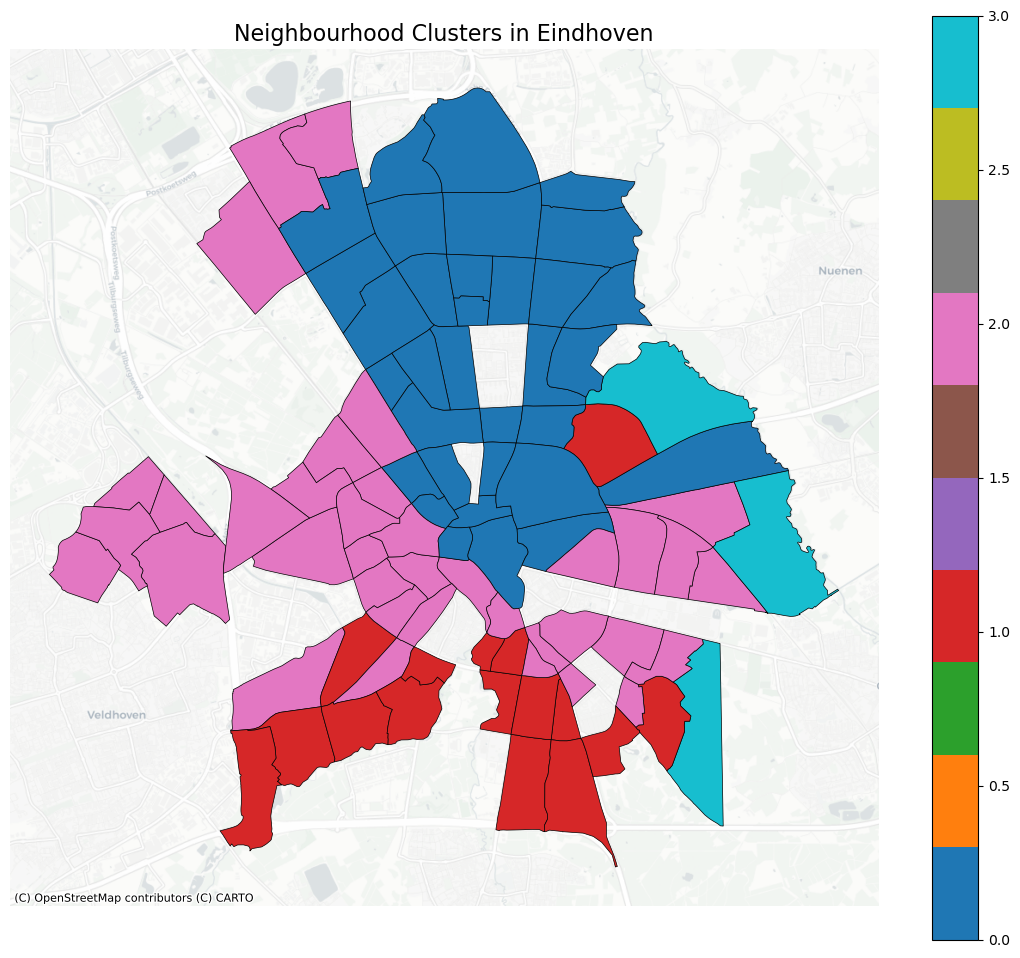
\includegraphics[width=0.45\textwidth]{../Images/kmeans_map.png}
        \caption{KMeans Clusters Map}
        \label{fig:kmeans_map}
    \end{figure}

    When fitting a Gradient Boosting Regressor and using SHapley Additive exPlanations (SHAP) values to explain the model, the following results were found:
    \begin{figure}[H]
        \centering
        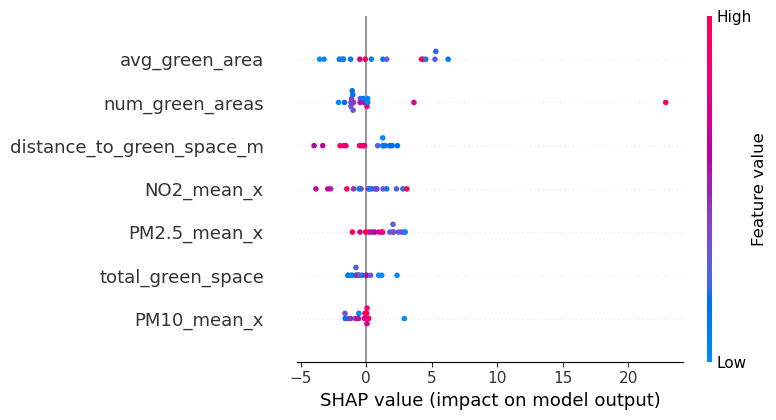
\includegraphics[width=0.45\textwidth]{../Images/shap_values.png}
        \caption{SHAP Values by Gradient Boosting Regressor}
        \label{fig:shap_values}
    \end{figure}
    Figure 4 shows the SHAP values, being a common method to explain machine learning models, which reveal that the most impactful features are the average size of a green area, the number of green areas and the distance to green spaces.
    Higher pollution raises predicted income, but results are mixed.
    When plotting the average levels of pollutents across neighbourhoods, the following results were found:
    \begin{figure}[H]
        \centering
        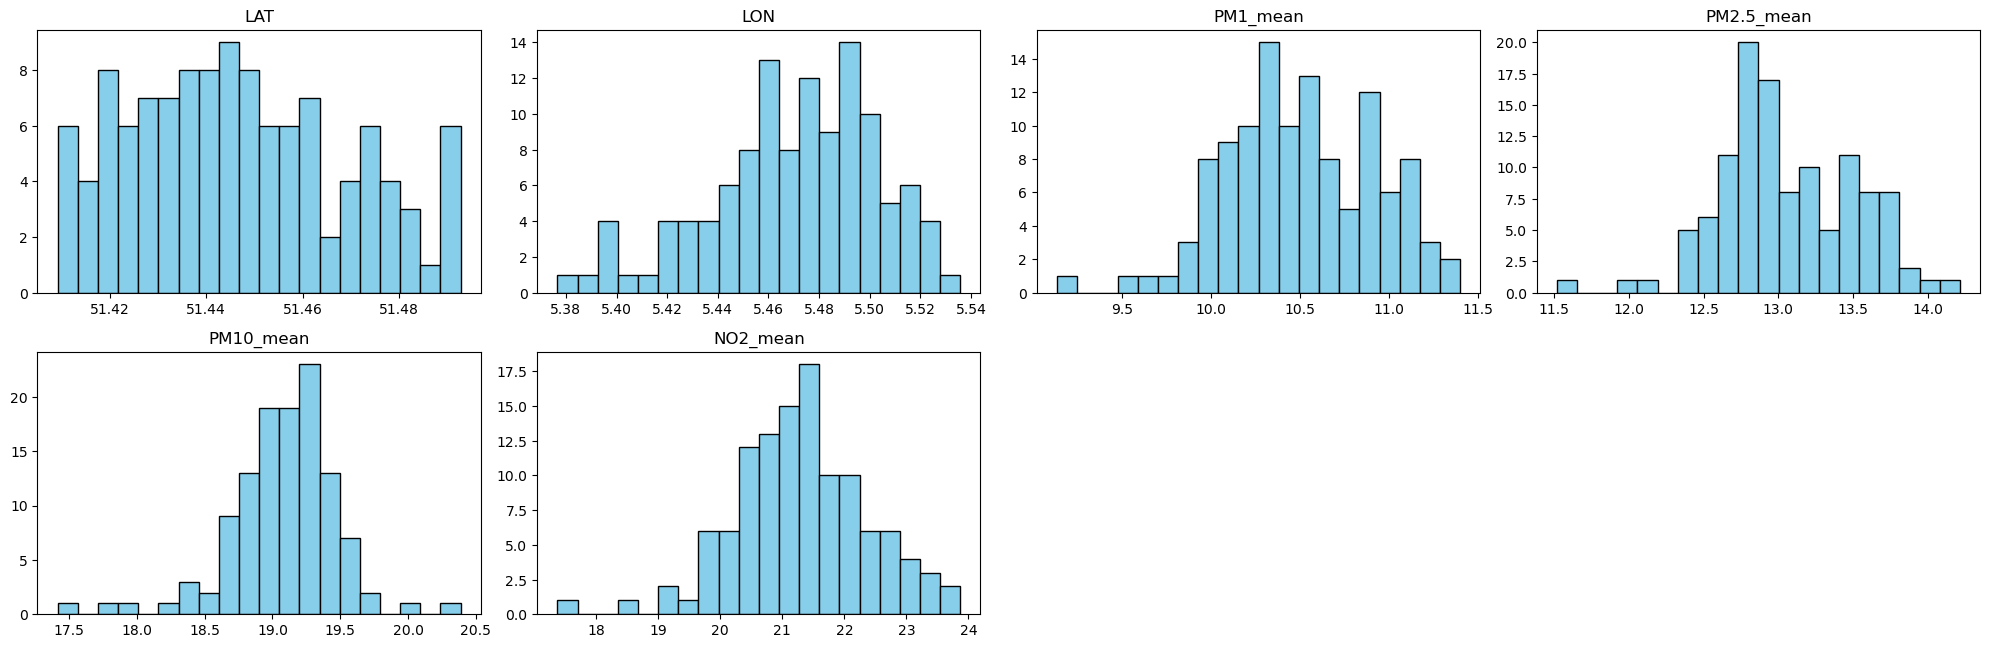
\includegraphics[width=0.45\textwidth]{../Images/pm25_per_neighborhood.png}
        \caption{Average PM2.5 per Neighborhood}
        \label{fig:pm25_per_neighborhood}
    \end{figure}
    The map shows that the average levels of PM2.5 and PM10 do not surpass the thresholds for dangerous levels; however, there are some neighborhoods that have higher levels of air pollution than others.
    These results are plotted against a map containing the threshholds for dangerous levels of PM2.5 and PM1, which are 35 $\mu$g/m\(^3\) (interim target 1); PM10, which is 70 $\mu$g/m\(^3\) (interim target 1, although it's worth mentioning that Eindhoven has reached interim target 3 and is on its way to achieve target 4); and lastly, NO2, which is 40 $\mu$g/m\(^3\) (interim target 1, although Eindhoven already reached Interim target 2) \cite{who2021aqg}.
    \section{Discussion}
    Based on the results, it is clear that there is a correlation between access to green spaces and income inequality, with lower income neighborhoods having less access to green spaces. However, it is not possible to generalise conclusion about air pollution and income. The results, especially outlined in Table 1, Figure 1 and Figure 4, do not show a clear correlation between air pollution and income in the neighborhoods of Eindhoven. However, as can be seen in Figures 2 and 3, there are neighbourhoods, particularly those clustered in Cluster 1, that are low income and have high levels of air pollution, although the significance of the cluster is mixed. 
    The models performed poorly overall, with the best performing model being the Random Forest Regressor, which achieved an $R^2$ of 0.02 and an RMSE of 16.57. The poor performance of the models can be attributed to the lack of some necessary additional features, such as public transport access, industrial factors and other factors. Furthermore, Exploratory Data Analysis revealed that air pollution, on average, does not surpass the threshold for harmful levels of PM2.5 and other metrics.
    However, it is important to note that Eindhoven, although having achieved impressive interim targets for air quality, still has some neighborhoods which haven't reached interim targets 4. If we account for these figures, the picture becomes more complex.
    \begin{figure}[H]
        \centering
        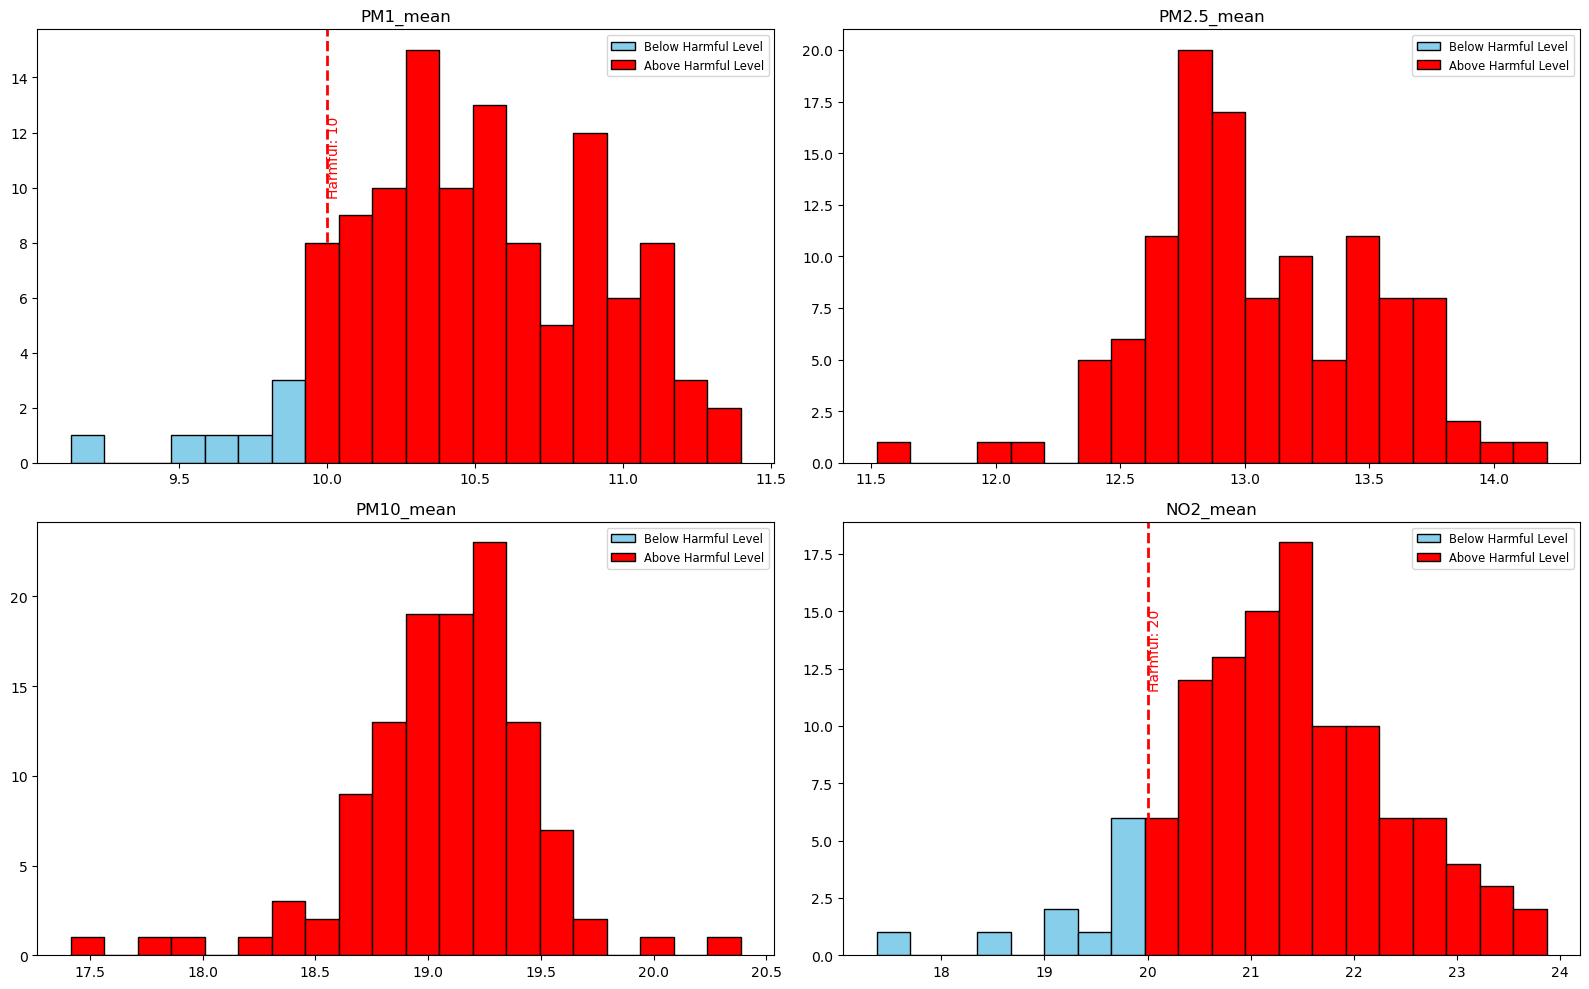
\includegraphics[width=0.45\textwidth]{../Images/interim_target_4.png}
        \caption{Average PM2.5 per Neighborhood}
        \label{fig:interim_target_4}
    \end{figure}
    If we take the advised values for the last target according to the WHO report, then Eindhoven still has a long way to go. The dicrease of air pollution can be done in multiple ways, some which the municipality already started by its own initiative to do, such as restricting the number and type of vehicles in the city centre \cite{eindhoven_zero_emissiezone}. But all pollutants must be reduced, being the most prominent the burning and collection of fossil fuels \cite{li2021spatiotemporal}.
    Despite no holistic correlation, there are still neighbourhoods that suffer from decreased air quality and suffer from economic strain. Their neighbourhoods necessitate further action from the local government in order to decrease wealth disparities. It has been prevously demonstrated that higher income communities tend to have lower climate resilience, including in exposure to PM2.5 \cite{li2023urban}, so it is hightly advised that the municipality maintaints a close watch to the status of these communities and combats the curb of inequality in relation to climate resilience in these spaces. Therefore, measures like electrification of housing infrastructure \cite{sierraclub2019electrification} and enlarging public transport access are necessary \cite{uttan2022climateresilient} (Eindhoven already has an electrified public transport fleet). The findings of this report that highlight inequalities mostly in the acces to green spaces also prove that these inequalities exist and the best way to stop them is to identify all the potential inequalities and factors and prevent them from happening in the first place. Access to green spaces and incidence of air pollution are intersectional with income inequality. In Eindhoven, air pollution is less of a problem. But this can change for better but also for worse, so it is deemed necessary to highlight this intersectionality.
    \linebreak
    A few ways that the local government can take action to mitigate the inequalities discussed in this report are:
    \begin{itemize}
        \item Increase access to green spaces in low income neighborhoods, by building more parks and green areas.
        \item Increase public transport access to green spaces so that people can easily reach them, especially in the periphery of city centre, especially those in south of the ring.
        \item Focus on measures which target low income neighbourhoods in net zero emissions and electrification plans.
        \item Increasing public transport capacity for lower income neighbourhoods for commuting.
        \item Turn neighborhoods into walkable, 15 minute neighborhoods, so that people can easily access green spaces and other amenities, either by walking or biking, which would decrease air pollution levels \cite{smartcities8020053}.
        \item Conduct further research on the topic in order to better understand the relation between air pollution, income inequality and access to green spaces.
        \item Faze out fossil fuels and achieve net zero emissions by 2050, as outlined in the Paris Agreement \cite{unfccc2015paris} while furthering the energy transition.
    \end{itemize}
    These measures would not only help to mitigate the inequalities discussed in this report but also improve the quality of life for all citizens of Eindhoven. It is ever more pressient to take action on issues of social justice and act locally so the implementation can be done in tandem with local communities, which know their city and its interests best.
    Another important aspect to consider is data availability and quality, as it was a challenge to find datasets which could complement this analysis. Additionally, some datasets, like the air pollution dataset, had significant hurdles associated with their aggregation. It is not favourable to resort to scraping an internet page and writing a script just to get historical data on air pollution, as it makes the work of the municipality less transparent and harder to research. Openness of data is important, as it allows for citizens and organisations to hold the local government accountable for its management.
    \section{Conclusion}
    In conclusion, this report has shown that there is a correlation between access to green spaces and income inequality in Eindhoven, with lower income neighborhoods having less access to green spaces. However, the results do not show a clear correlation between air pollution and income in the neighborhoods of Eindhoven. The models performed poorly overall, with the best performing model being the Random Forest Regressor, which achieved an $R^2$ of 0.02 and an RMSE of 16.57. The poor performance of the models can be attributed to the lack of some necessary additional features, such as public transport access, industrial factors and other factors.
    Despite the lack of a clear correlation between air pollution and income, there are still neighborhoods that suffer from decreased air quality and suffer from economic strain. These neighborhoods necessitate further action from the local government in order to decrease wealth disparities.
    The report has also outlined a few ways that the local government can take action to mitigate the inequalities discussed in this report, such as increasing access to green spaces in low income neighborhoods, increasing public transport access to green spaces, focusing on measures which target low income neighborhoods in net zero emissions and electrification plans, increasing public transport capacity for lower income neighborhoods for commuting, turning neighborhoods into walkable, 15 minute neighborhoods, conducting further research on the topic and phasing out fossil fuels and achieving net zero emissions by 2050.
    These measures would not only help to mitigate the inequalities discussed in this report but also improve the quality of life for all citizens of Eindhoven. 

    \section{Maintainability Statement}
    All material in this report, including code and clean datasets, are available in the GitHub repository \url{https://github.com/GuiOliv/EindhovenClimateInequality}. The code is written in Python and uses the Pandas, NumPy, Scikit-learn, Matplotlib and Seaborn libraries. The report is written in LaTeX and can be compiled using any LaTeX editor.
    Read the README file in the repository for more information on its contents.
    This project also utilised a scrum board tool hosted by Zenkit, which can be accessed at \url{https://public.zenkit.com/c/uVzZR_LpqQ/eindhoven-inequality?v=WCKFdeMBERSa}. The board contains all the tasks and issues that were created during the project, along with their status and progress. Each item will have a time and date for when they were added and completed. The tasks related to the datasets will also contain such datasets and sources.
\end{multicols}

\bibliographystyle{plain}
\bibliography{sources}

\appendix
\section*{Appendix: Figures}

\begin{figure}[H]
    \centering
    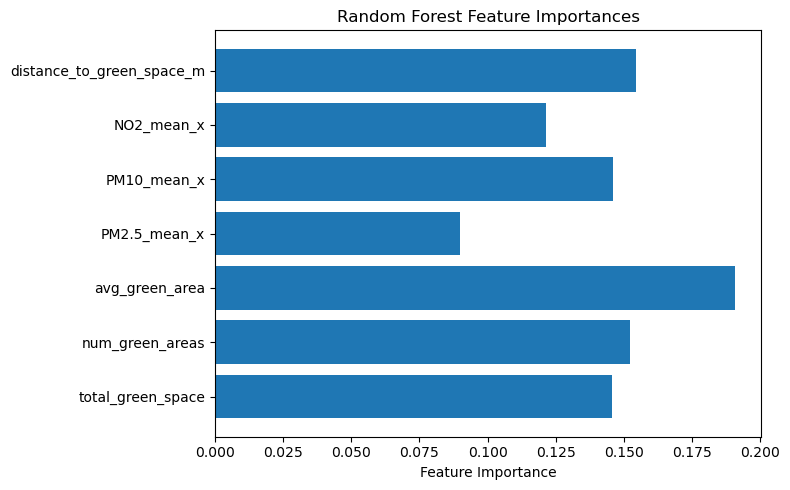
\includegraphics[width=0.6\textwidth]{../Images/feature_importance.png}
    \caption{Feature importance by Random Forest Regressor (duplicate of Figure~\ref{fig:feature_importance})}
    \label{fig:feature_importance_appendix}
\end{figure}

\begin{figure}[H]
    \centering
    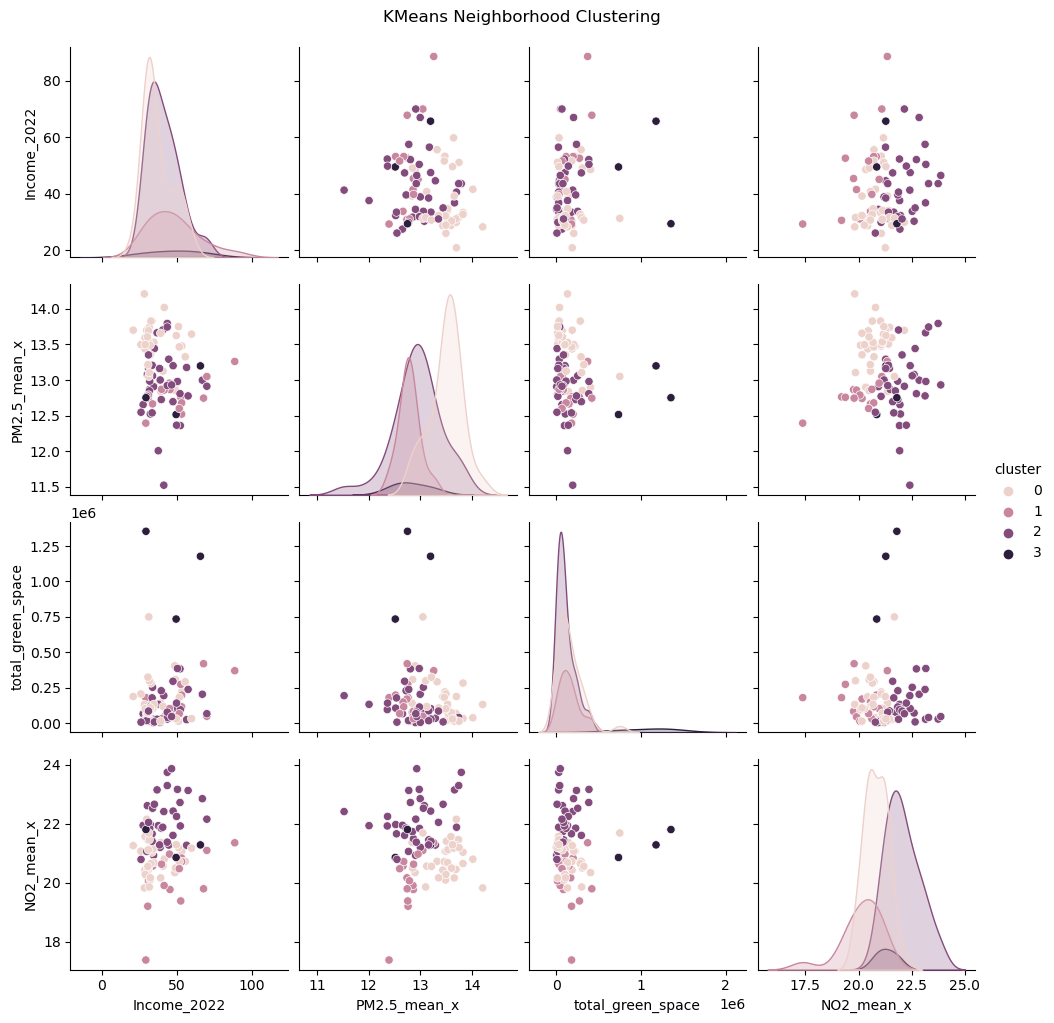
\includegraphics[width=0.6\textwidth]{../Images/kmeans_clusters.png}
    \caption{KMeans Clusters (duplicate of Figure~\ref{fig:kmeans_clusters})}
    \label{fig:kmeans_clusters_appendix}
\end{figure}

\begin{figure}[H]
    \centering
    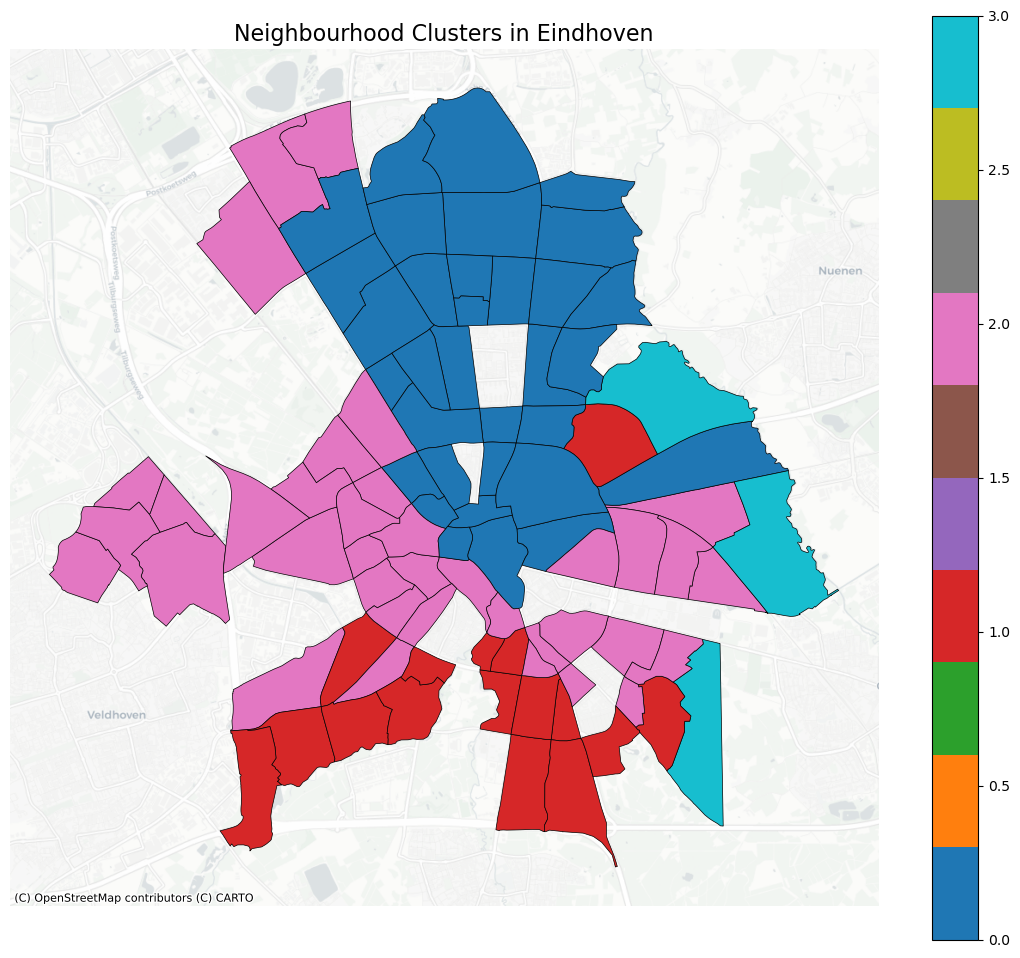
\includegraphics[width=0.6\textwidth]{../Images/kmeans_map.png}
    \caption{KMeans Clusters Map (duplicate of Figure~\ref{fig:kmeans_map})}
    \label{fig:kmeans_map_appendix}
\end{figure}

\begin{figure}[H]
    \centering
    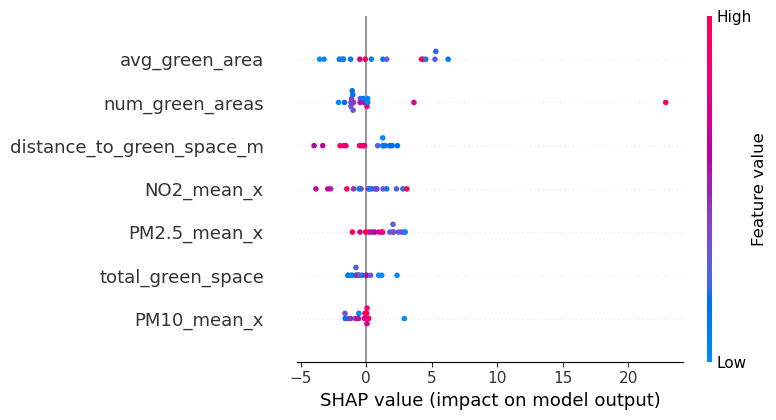
\includegraphics[width=0.6\textwidth]{../Images/shap_values.png}
    \caption{SHAP Values by Gradient Boosting Regressor (duplicate of Figure~\ref{fig:shap_values})}
    \label{fig:shap_values_appendix}
\end{figure}

\begin{figure}[H]
    \centering
    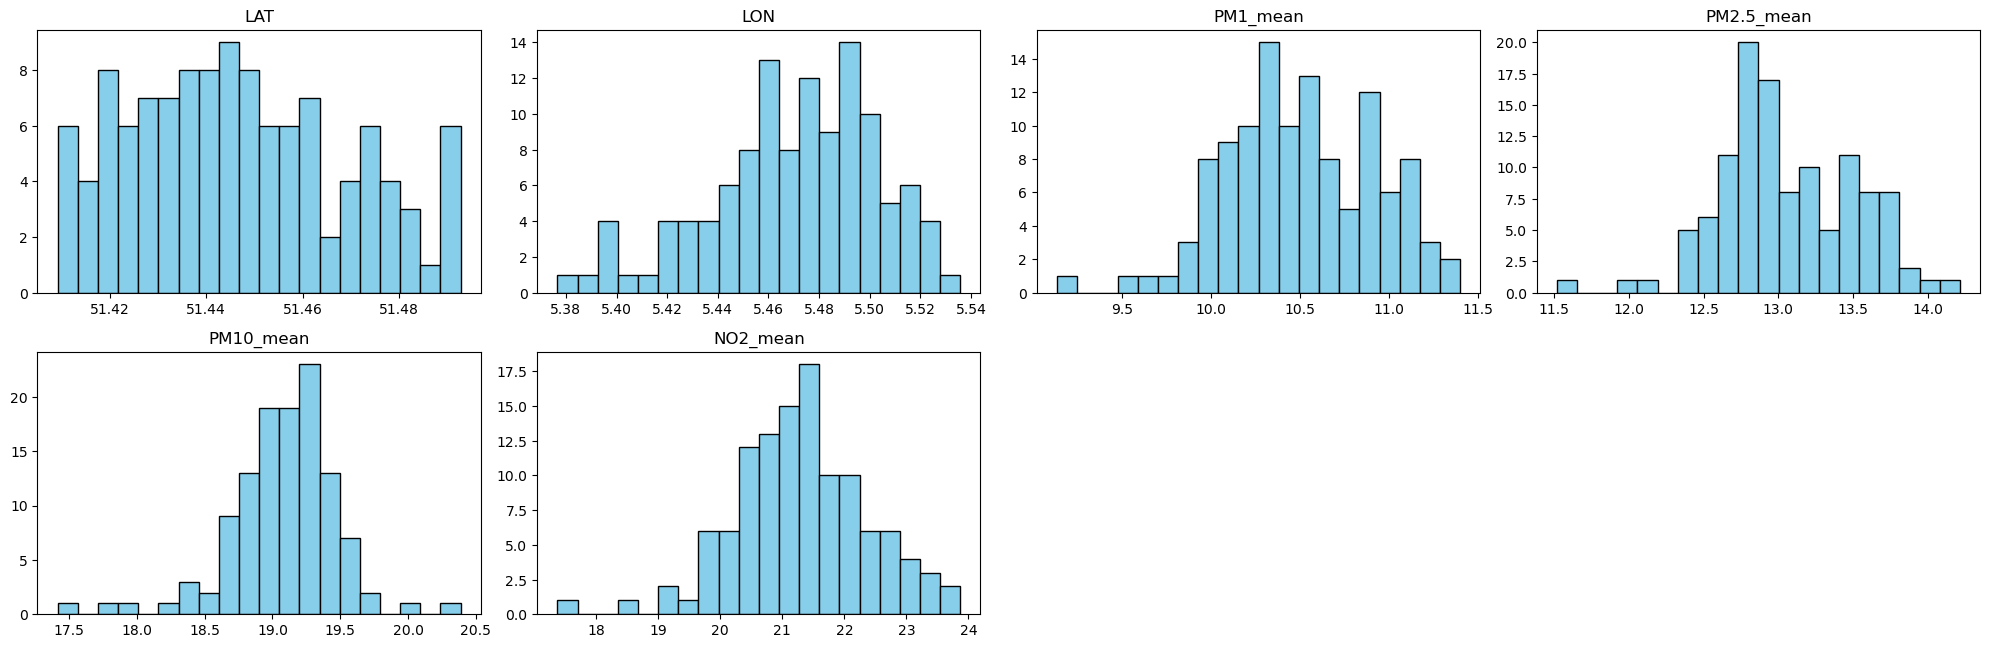
\includegraphics[width=0.6\textwidth]{../Images/pm25_per_neighborhood.png}
    \caption{Average PM2.5 per Neighborhood (duplicate of Figure~\ref{fig:pm25_per_neighborhood})}
    \label{fig:pm25_per_neighborhood_appendix}
\end{figure}

\begin{figure}[H]
    \centering
    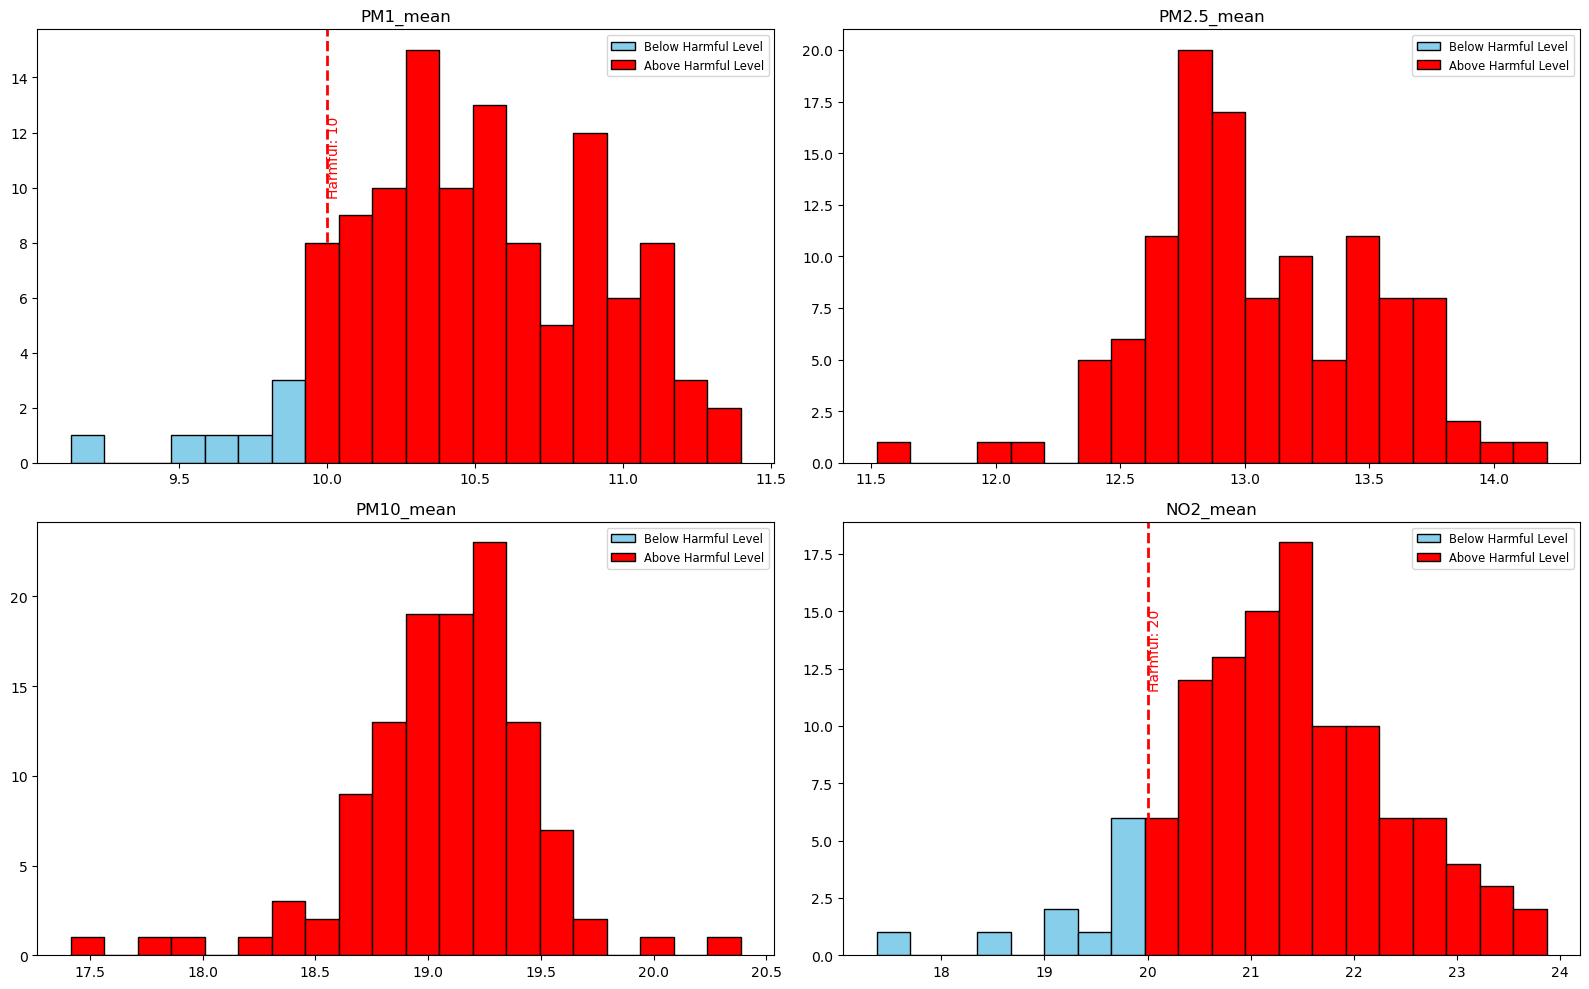
\includegraphics[width=0.6\textwidth]{../Images/interim_target_4.png}
    \caption{Average PM2.5 per Neighborhood (duplicate of Figure~\ref{fig:interim_target_4})}
    \label{fig:interim_target_4_appendix}
\end{figure}

\end{document}